also% Work done: ember production by burning vegetation near buildings (Gatlinburg, Chimney Tops 2, 2016)
% Needs in the preamble: \usepackage{graphicx,booktabs,amsmath,siunitx}
% Figures are in figures/ next to this file.

\section{Work done: ember production by vegetation near buildings}
\label{sec:ember_production}

\subsection{Aim}
Objective~2 needs the number of embers that a burning vegetation cell produces next to a building,
as the source term for the probability of ember accumulation on a sloped roof. This section estimates
that number for the Gatlinburg part of the 2016 Chimney Tops~2 fire with ELMFIRE~v1.1. Buildings are
made non-burnable, so every ember counted comes from vegetation, not from burning houses.

\subsection{Model}
ELMFIRE is a two-dimensional raster fire model. It is not a CFD model: wind is an input and the fire
does not feed back on the atmosphere. The fire front is a level set $\phi(x,y,t)$ ($\phi<0$ burned),
moved by the local spread rate:
\begin{equation}
  \frac{\partial \phi}{\partial t} + \mathbf{U}\cdot\nabla\phi = 0 ,
  \label{eq:levelset}
\end{equation}
where $\mathbf{U}$ is the spread velocity. Its magnitude in the head-fire direction is the Rothermel
(1972) rate of spread,
\begin{equation}
  R = \frac{I_R\,\xi\,(1+\phi_w+\phi_s)}{\rho_b\,\varepsilon\,Q_{ig}} ,
  \label{eq:rothermel}
\end{equation}
with $R$ the rate of spread (\si{\metre\per\second}), $I_R$ the reaction intensity
(\si{\kilo\watt\per\square\metre}), $\xi$ the propagating flux ratio (--), $\phi_w$ and $\phi_s$ the
wind and slope factors (--), $\rho_b$ the oven-dry bulk density (\si{\kilo\gram\per\cubic\metre}),
$\varepsilon$ the effective heating number (--) and $Q_{ig}$ the heat of pre-ignition
(\si{\kilo\joule\per\kilo\gram}). The fireline intensity of each burning cell is Byram's
\begin{equation}
  I = H\,w_a\,R \qquad [\si{\kilo\watt\per\metre}],
  \label{eq:byram}
\end{equation}
with $H$ the heat content and $w_a$ the fuel consumed per unit area.

\paragraph{Ember generation.} With the \texttt{PER-MW} generation model, a burning vegetation cell
of width $\Delta x$ emits embers at a rate proportional to its fire power:
\begin{equation}
  \dot N_e = \frac{I\,\Delta x}{1000}\,G_v \qquad [\text{embers}\,\si{\per\second}],
  \label{eq:genrate}
\end{equation}
where $I\,\Delta x/1000$ is the fire power of the cell in MW and $G_v = 33.3$ embers
\si{\per\second\per\mega\watt} is the ELMFIRE default yield for vegetation. Emission lasts
$\tau_{eg} = \SI{10}{\second}$ after the fire arrives in the cell, so the embers produced by one cell are
\begin{equation}
  N_e = \dot N_e\,\tau_{eg} = \frac{I \times 30 \times 33.3}{1000}\times 10 \;\approx\; 10\,I ,
  \label{eq:gen}
\end{equation}
with $I$ in \si{\kilo\watt\per\metre} and $\Delta x = \SI{30}{\metre}$. Equation~\eqref{eq:gen} is the
amount the model intends to emit. It is calculated from the fireline-intensity output, because ELMFIRE
writes no per-cell generation map for the Eulerian ember model.

\paragraph{Transport and landing.} Embers are carried downwind with the \texttt{EMPIRICAL}
(lognormal) spotting-distance model and counted on the grid with the \texttt{EULERIAN} accumulation
model. Generation and transport are deterministic. The only random step is ignition by landed embers
(\texttt{PHYSICAL} model): in a time step $\Delta t$ a cell ignites with probability
\begin{equation}
  P_N = 1-(1-P_{ign})^{\Delta t/\tau_{ign}} ,
  \label{eq:pign}
\end{equation}
with $P_{ign}=0.9$ and $\tau_{ign} = \SI{30}{\second}$ for vegetation. If the landed count is wanted as a
load, it is $L = N_{land}\,m_e/\Delta x^2$, with $m_e = \SI{0.2}{\gram}$ per ember and
$\Delta x^2 = \SI{900}{\metre\squared}$.

\subsection{Inputs}
Table~\ref{tab:inputs} lists the inputs. Fuels are the LANDFIRE~1.4.0 (about 2014, before the fire)
Scott and Burgan 40 fuel models, prepared with the CloudFire tool on a \SI{40}{\kilo\metre} square domain
at \SI{30}{\metre}. In the domain the main fuels are TL6 (moderate-load broadleaf litter, 49.4\,\% of
cells), TL2 (low-load broadleaf litter, 37.1\,\%), TU5 (very high-load timber-shrub, 5.2\,\%),
GR2 (1.3\,\%), TU2 (0.9\,\%) and TL3 (0.7\,\%); 2.3\,\% is non-burnable (NB9). Building footprints
(Microsoft US Building Footprints) were placed on the grid: a cell with a footprint fraction of at least
0.02 became a building cell (fuel 91, 28{,}060 cells), and the LANDFIRE 91 cells without buildings
(roads, parking) became non-burnable (99). With \texttt{USE\_BLDG\_SPREAD\_MODEL = .FALSE.} building
cells cannot burn, but embers still land on them.

\begin{table}[htbp]
  \centering
  \caption{Inputs of the non-burnable-building runs.}
  \label{tab:inputs}
  \small
  \begin{tabular}{@{}lp{0.62\textwidth}@{}}
    \toprule
    Input & Value \\
    \midrule
    Model & ELMFIRE v1.1 \\
    Domain, grid & $\SI{40}{\kilo\metre}\times\SI{40}{\kilo\metre}$, \SI{30}{\metre} cells (UTM 17N) \\
    Fuel & LANDFIRE 1.4.0, FBFM40 (CloudFire) \\
    Buildings & Microsoft footprints, fuel 91, non-burnable \\
    Weather & CloudFire historical, hourly, \SI{600}{\metre} grid \\
    Wind over the town (20 ft) & 14--32 mph hourly mean, up to 42 mph in single cells, from SSE (160--180\si{\degree}) \\
    Dead fuel moisture & 1-h 8--60\,\%, 10-h 9--39\,\%, 100-h 11--18\,\% (CloudFire) \\
    Live fuel moisture & herbaceous 30\,\%, woody 60\,\% \\
    Ignition & spot fire 2: 1-acre circle at \ang{35.690}N, \ang{83.497}W, \\
             & and the same circle moved 1 km N, S, E and W \\
    Start, duration & 28 Nov 2016 11:00 EST, 16 h \\
    Time step & 30 s maximum, CFL 0.4 \\
    Spotting & \texttt{PER-MW}, \texttt{EMPIRICAL}, \texttt{EULERIAN}, \texttt{PHYSICAL} \\
             & critical intensity 0, 100\,\% of burning cells spot, $\tau_{eg}=\SI{10}{\second}$ \\
    Runs & one run (seed 1) per ignition location \\
    \bottomrule
  \end{tabular}
\end{table}

One run per location is enough here. Generation and transport are deterministic, so the seed changes
only which landed embers ignite new cells, and therefore which cells burn. The distribution of embers
produced per cell next to buildings was the same for the five runs (one per location) as for all
fifty runs (ten per location): median 169 against 166 embers, 90th percentile 595 against 588.

\subsection{Buildings and fire perimeter}
\paragraph{Fire perimeter.} The burned area is the final perimeter of the Chimney Tops~2 fire from the
Monitoring Trends in Burn Severity (MTBS) programme (fire ID TN3563108347820161123, 15{,}003~acres on the
model grid). It is drawn as a black line in Figs.~\ref{fig:spread} and~\ref{fig:production}.

\paragraph{Buildings.} Building footprints are the Microsoft US Building Footprints (polygons, imagery
captured September--December 2019). They give the building cells of the model grid
and the 1{,}614 buildings whose centroid lies inside the MTBS perimeter, which are the buildings analysed
here. Because the footprints were mapped after the fire, each building inside the perimeter was labelled
from NAIP aerial imagery taken before (17--18 April 2016) and after the fire (30 October 2018), at 1~m
resolution: an automatic first pass compared the roof in the two years (NDVI, colour change and pixel
correlation), and every building was then checked by eye. The result is 404 buildings destroyed or
damaged, 984 that survived, and 226 left out (built after the fire, or unclear). These 1{,}388 labelled
buildings are the ones used in Tables~\ref{tab:production} and~\ref{tab:ignition}.

\subsection{Results}

\paragraph{Fire spread.} Figure~\ref{fig:spread} shows the time of arrival for the five ignition
locations. From each ignition the fire runs north-northwest, pushed by the south-southeasterly wind.
For the first nine hours it grows slowly (reported location: 110~acres after 1~h, 910~acres after 9~h).
Between 10 and 11~h (21:00--22:00 EST), when the wind over the town is strongest, it jumps from
1{,}485 to 5{,}947~acres; the large areas of one colour show many cells lit at the same time by
embers landing ahead of the front. The fire burned 6{,}693 (reported), 8{,}105 (1~km north),
6{,}222 (1~km south), 9{,}681 (1~km east) and 610~acres (1~km west). The west fire stops at the
Parkway, where most cells are buildings or roads and so cannot burn. In all runs the fire passes
through the eastern half of the town and never reaches the western part.

\begin{figure}[htbp]
  \centering
  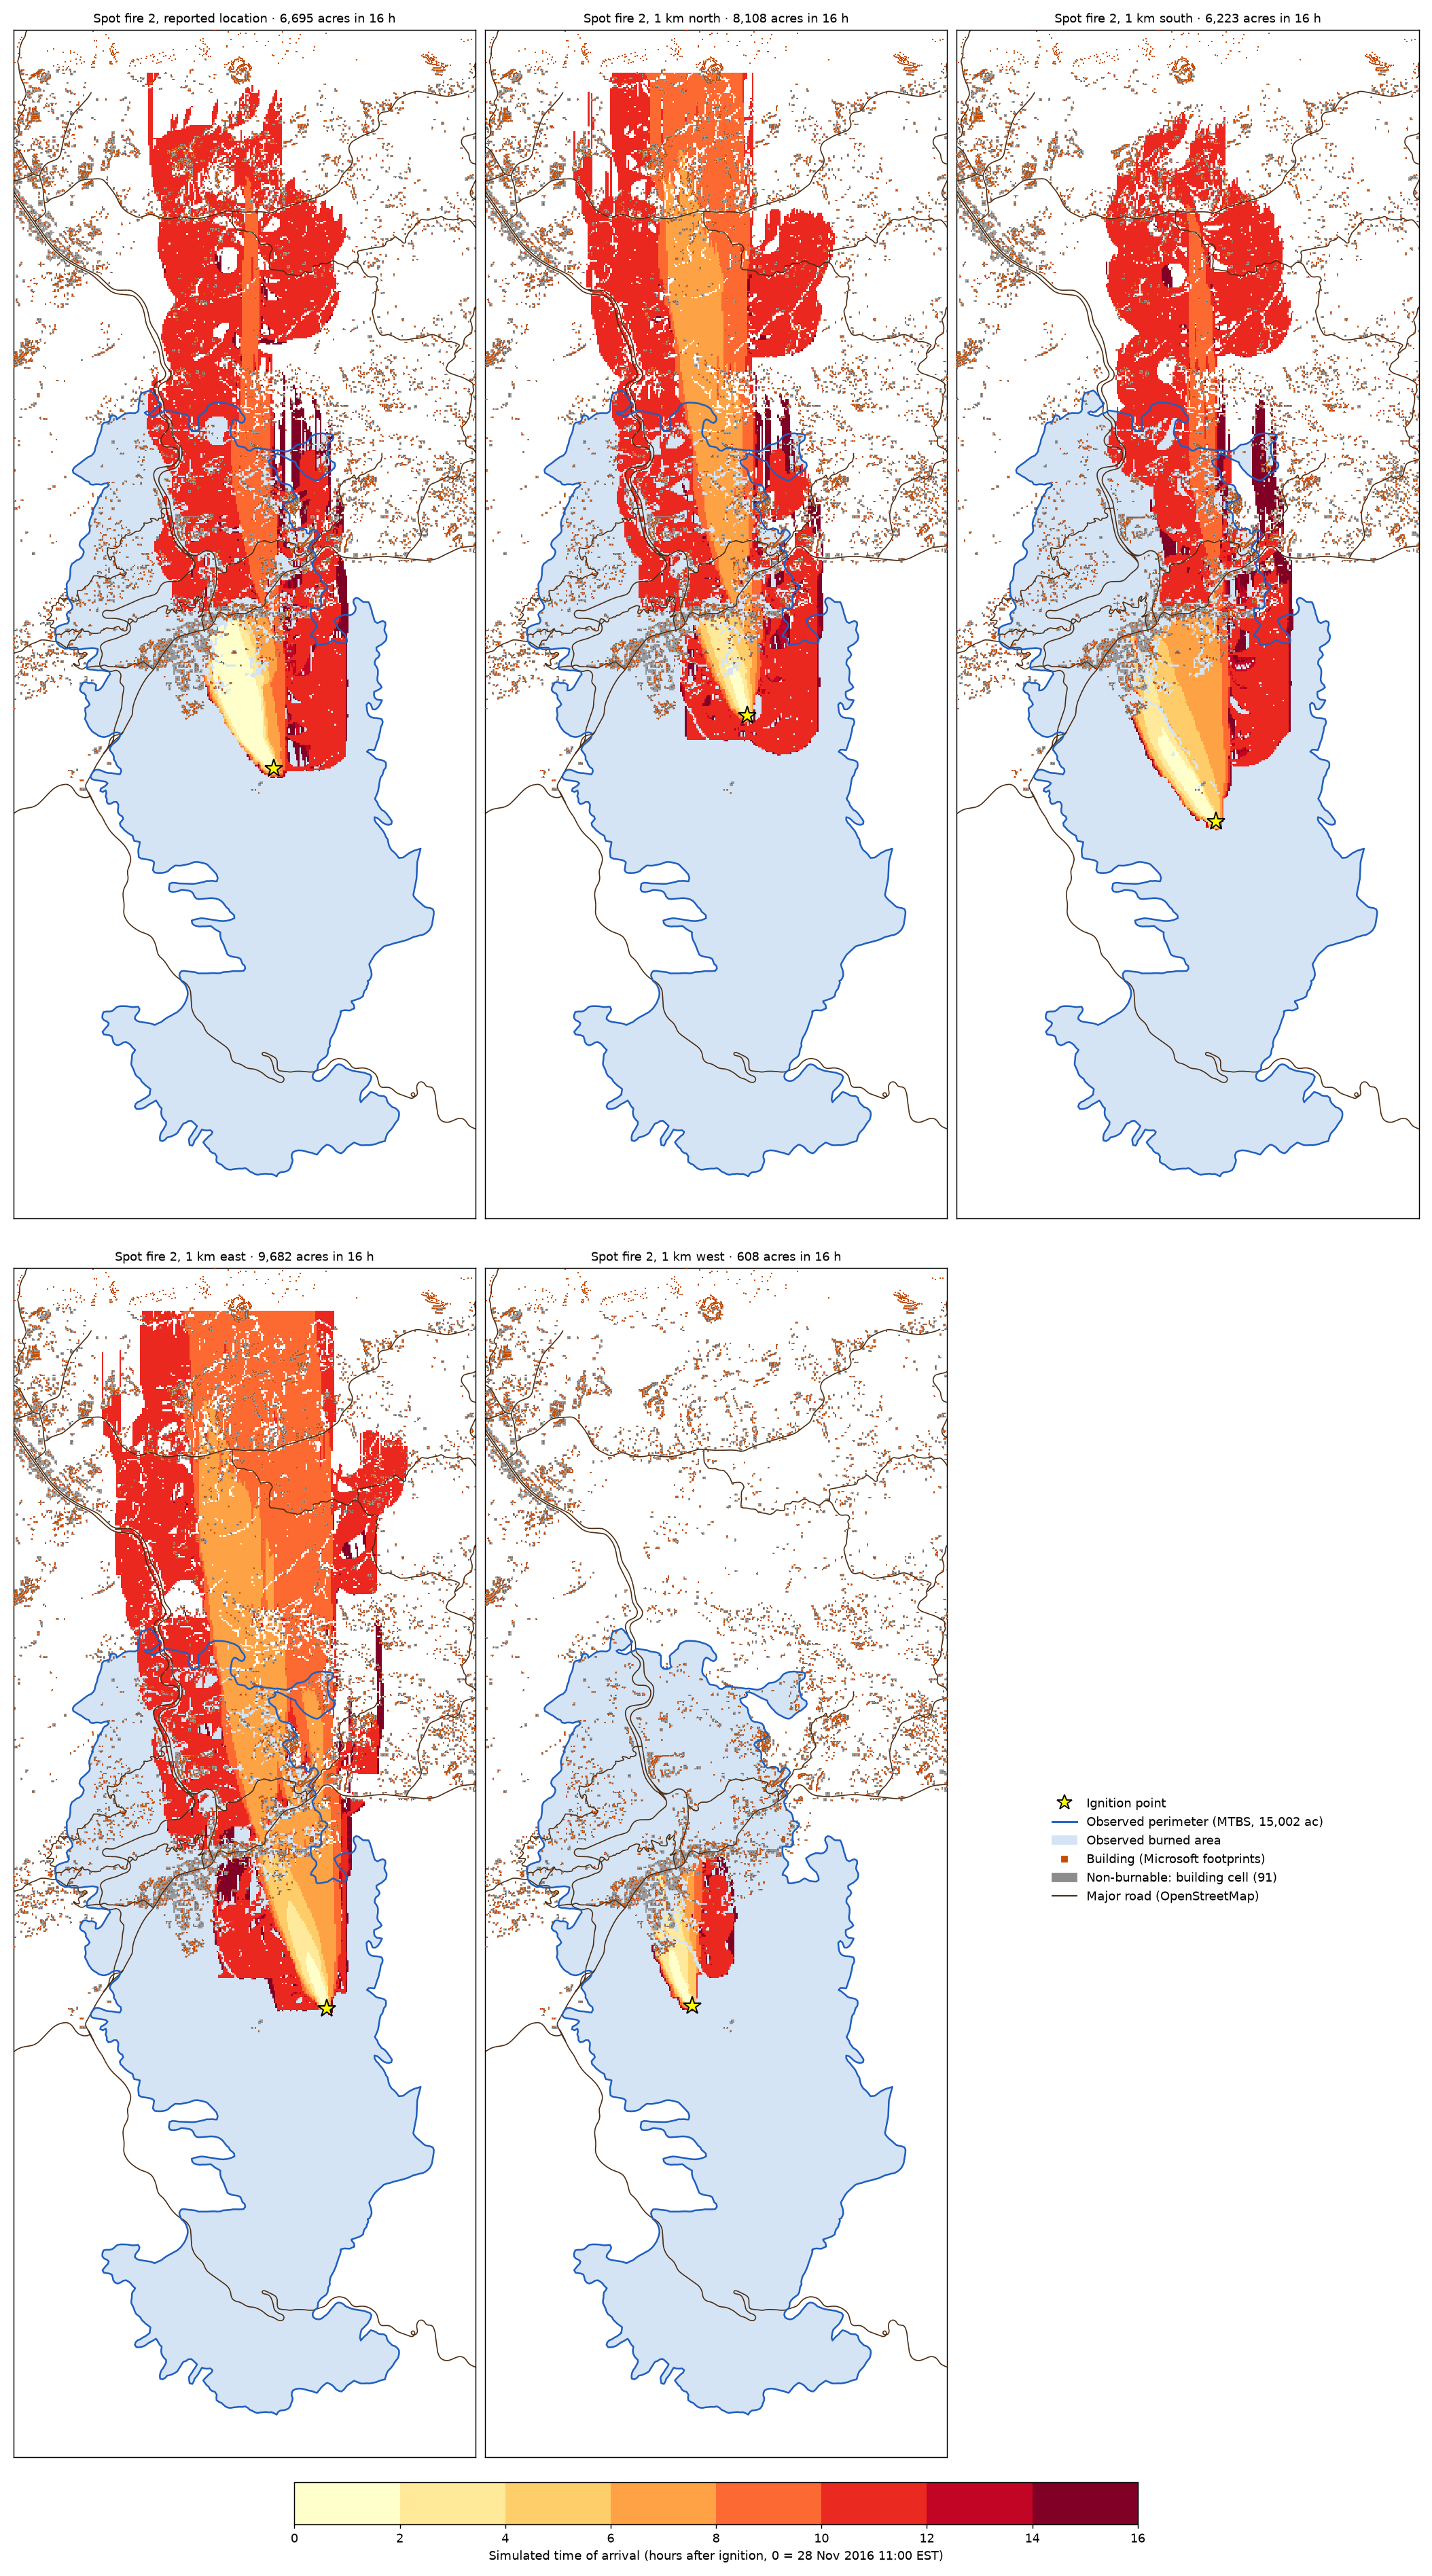
\includegraphics[width=\textwidth]{figures/fire_spread_seed1.png}
  \caption{Fire spread (time of arrival, hours after 28 Nov 2016 11:00 EST) for the reported spot-fire
  location and the four 1~km shifts, buildings non-burnable, seed 1. White lines: fire front every 2~h;
  star: ignition; red dots: buildings; black line: MTBS perimeter.}
  \label{fig:spread}
\end{figure}

\paragraph{Ember production.} Figure~\ref{fig:production} maps the embers produced by each burned
vegetation cell, from Eq.~\eqref{eq:gen}. Table~\ref{tab:production} gives the distribution for the
vegetation cells next to a building (the 8 neighbouring cells). For four of the five locations the
median is 160--190 embers per cell and the 90th percentile about 580--620 embers; the west location
gives a median of 83. The spread is wide: 10\,\% of cells produce fewer than 18 embers and 1\,\% more
than about 14{,}000. The production per cell is set by the local fireline intensity
(Eq.~\eqref{eq:byram}), so it depends on the fuel and the wind at the time the fire arrives, and much
less on where the fire started.

\begin{figure}[htbp]
  \centering
  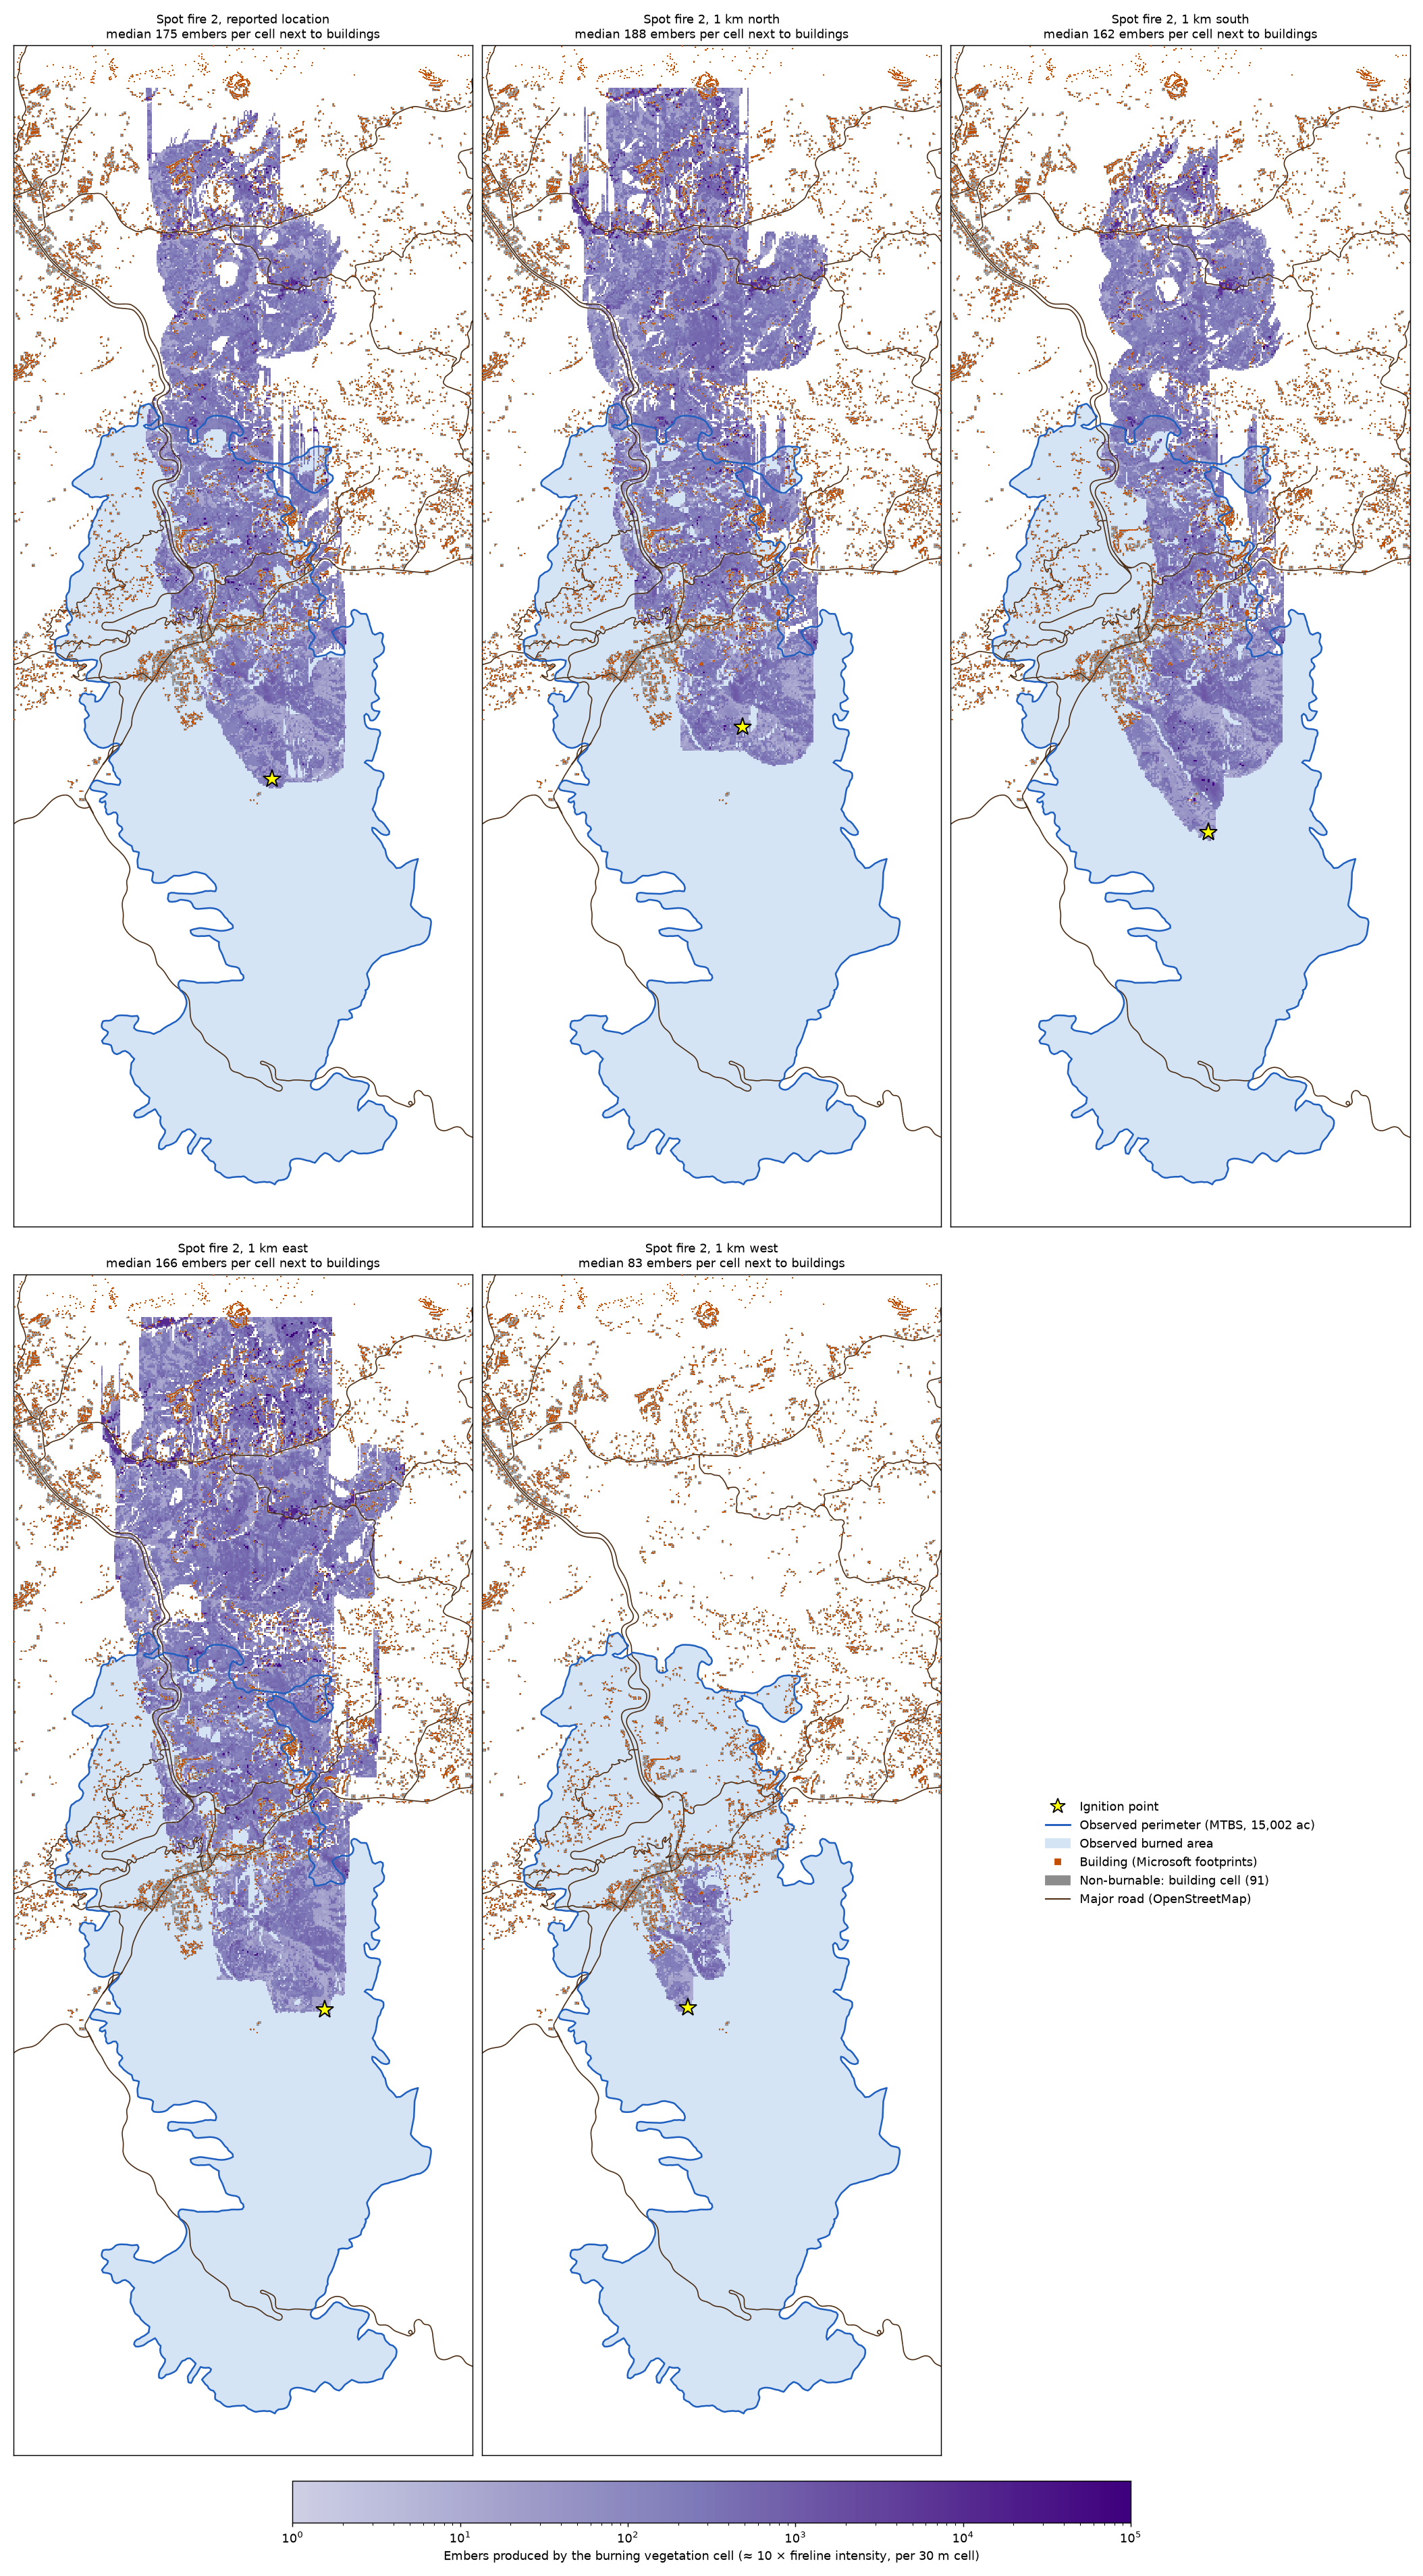
\includegraphics[width=\textwidth]{figures/ember_production_seed1.png}
  \caption{Embers produced by each burned vegetation cell ($N_e \approx 10\,I$, per 30~m cell, log
  scale) for the five ignition locations, buildings non-burnable, seed 1. Blue dots: buildings;
  black line: MTBS perimeter.}
  \label{fig:production}
\end{figure}

\begin{table}[htbp]
  \centering
  \caption{Embers produced per burned vegetation cell next to a building (8 neighbouring cells), seed 1.}
  \label{tab:production}
  \small
  \begin{tabular}{@{}lrrrrrr@{}}
    \toprule
    Ignition & Veg.\ cells burned & Cells next to buildings & P10 & Median & P90 & P99 \\
    \midrule
    Reported    & 30{,}102 & 1{,}581 & 17 & 176 & 577 & 15{,}821 \\
    1 km north  & 36{,}456 & 1{,}610 & 18 & 188 & 588 & 14{,}642 \\
    1 km south  & 27{,}980 & 1{,}368 & 18 & 162 & 589 & 13{,}864 \\
    1 km east   & 43{,}537 & 1{,}701 & 18 & 167 & 625 & 14{,}336 \\
    1 km west   &  2{,}736 &   247   &  0 &  83 & 500 & 33{,}119 \\
    \bottomrule
  \end{tabular}
\end{table}

\paragraph{Ember ignitions next to buildings.} ELMFIRE records which cells were ignited by landed
embers rather than reached by the spreading front (\texttt{DUMP\_EMBER\_IGNITION}). Of the 3{,}213
vegetation cells next to buildings, Table~\ref{tab:ignition} gives, for each ignition location, how many
burned, how many of those were ignited by embers, and the average number of embers they then produced
(Eq.~\eqref{eq:gen}). In every direction most of the burned cells next to buildings were ignited by
embers, and they produced on average 2{,}000--3{,}000 embers per cell.

\begin{table}[htbp]
  \centering
  \caption{Vegetation cells next to buildings (8 neighbouring cells, 3{,}213 cells): cells ignited by
  embers and embers produced per burned cell, seed 1.}
  \label{tab:ignition}
  \small
  \begin{tabular}{@{}lrrr@{}}
    \toprule
    Ignition & Burned & Ignited by embers & Mean embers \\
             & cells  & (cells)           & per cell    \\
    \midrule
    Observed    & 1{,}581 & 1{,}462 & 2{,}963 \\
    1 km north  & 1{,}610 & 1{,}482 & 2{,}312 \\
    1 km south  & 1{,}368 & 1{,}271 & 2{,}165 \\
    1 km east   & 1{,}701 & 1{,}567 & 2{,}132 \\
    1 km west   &   247   &   222   & 1{,}989 \\
    \bottomrule
  \end{tabular}
\end{table}

\subsection{Limitations}
\begin{itemize}
  \item Equation~\eqref{eq:gen} is the intended emission. The model only emits over the part of the
        10~s window that overlaps its time steps (up to 30~s), so the embers that actually land are
        0.26--0.53 of this amount in the runs checked.
  \item The intensity output includes canopy fire, while generation uses the surface fire only, so
        cells with crown fire are over-estimated (this affects the top 1\,\%).
  \item The yield $G_v = 33.3$ embers \si{\per\second\per\mega\watt} and the ember mass of 0.2~g are
        ELMFIRE defaults, not values measured for these fuels.
  \item With non-burnable buildings the fire does not spread through the town, so the western cluster
        of destroyed buildings is never reached; the numbers describe vegetation-to-building exposure only.
\end{itemize}
